%        File: report.tex
%     Created: Sat Jan 19 07:00 AM 2013 J
% Last Change: Sat Jan 19 07:00 AM 2013 J
%
\documentclass[a4paper,12pt,titlepage]{jreport}
\usepackage[dvips]{graphicx}
\usepackage{amsmath}
\usepackage{ascmac,here,txfonts,txfonts}
\usepackage{listings}
\usepackage{color}
\usepackage{fancybox} 

\lstset{
breaklines = true,
language=C++,
basicstyle=\ttfamily\scriptsize,
commentstyle={\itshape \color[cmyk]{1,0.4,1,0}},
classoffset=1,
keywordstyle={\bfseries \color[rgb]{0,0,1}},
stringstyle={\ttfamily \color[rgb]{0,0,1}},
frame=tRBl,
framesep=5pt,
showstringspaces=false,
numbers=left,
stepnumber=1,
numberstyle=\tiny,
tabsize=2,
}

% 年度名
\def\@yearname{%
\def\@heisei{\year}%
\advance\@heisei-1988%
\ifnum \month<4 \advance\@heisei-1 \fi%
平成%
\ifnum \@heisei=1 元%
\else \number\@heisei%
\fi%
年度\ \@thesisname
}

\renewcommand{\maketitle}{%
\begin{titlepage}%
  \let\footnotesize\small%
  \let\footnoterule\relax%
  \let\footnote\thanks%
  \null\vfil%
  % \vskip 60\p@%
  \begin{center}%
    {\Large 平成25年度 卒業論文 \par}%
    \vskip 1em%
    {\LARGE クラウドソーシングを用いたゲームのレベルデザイン効率化 \par}%
    \vskip 1em%
    {\LARGE \textit{Improvement of game level-design via Crowdsourcing.} \par}%
    \vskip 12em%
    \vskip 1em%
    \lineskip .75em%
    {\Large 北海道大学 \hskip .5em 工学部 \par}
    \vskip .0em
    {\Large 情報エレクトロニクス系 \hskip .5em 情報工学コース \par}
    \vskip .0em
    {\Large 複雑系工学講座 \hskip .5em 表現系工学研究室 \par}
    \vskip 1.0em%
    {\Large 三木 康暉 \par}%
    \vskip 1.5em%
    {\Large 平成25年2月14日 \par}%   
  \end{center}\par%
  % \@thanks\vfil\null%
  \end{titlepage}%
}

%%%%%%%%%%%%%%%%%%%%%%%%%%%%
% layout

\renewcommand{\baselinestretch}{1.15}

\setlength{\paperwidth}{597pt}
\setlength{\paperheight}{845pt}

\setlength{\hoffset}{10pt}
\setlength{\voffset}{10pt}
\setlength{\topmargin}{0pt}
\setlength{\headheight}{0pt}
\setlength{\headsep}{0pt}
\setlength{\topskip}{0pt}
\setlength{\oddsidemargin}{0pt}
\setlength{\evensidemargin}{0pt}
\setlength{\marginparwidth}{72pt}
\setlength{\marginparsep}{10pt}
\setlength{\textwidth}{433pt}  % paperwidth - (hoffset + 72pt) - (marginparwidth + marginparsep)
%\setlength{\textheight}{681pt} % paperheight - ((voffset + 72pt) * 2)
\setlength{\textheight}{672pt} %

%\setlength{\footskip}{41pt} 
\setlength{\footskip}{50pt}    % 本文とフッタ領域の間隔

\title{タイトル}
% \author{三木 康暉}
% \thesisname{卒業論文}
% \univname{北海道大学}
% \facultyname{工学部}
% \deptname{情報エレクトロニクス学科}
% \coursename{情報工学コース}
% \fieldname{複雑系工学講座}
% \labname{表現系工学研究室}
 \date{平成25年2月14日}
% 
\begin{document}
\maketitle
\clearpage


\pagenumbering{roman}
\tableofcontents
\pagebreak
\pagenumbering{arabic}

%マジで書くことがないのでここが行数を稼ぎたい 目標:3枚
\chapter{はじめに}
\section{研究背景}
今日、日々、商用、非商用問わず多数のゲーム作品が世に生み出され続けている。
開発環境のオープン化と一般化が進み、個人でも簡単にゲーム作品を世に輩出することが可能になったことが一因としてあげられる。

同時に、世に出回るゲーム作品が増えたことで、商品として要求されるゲームの質、物量が一昔前と比べると、格段に肥大化し続けている。
重厚長大化するゲーム作品が求められることで、ゲーム開発はますます複雑化し、多数の人手、多額の資金、長期の開発期間、熟練された開発ノウハウが求められるようになってきた。

その一方で、ゲーム作品の単価は急速に低下しており、一作品数千円というパッケージ販売の時代から、一作品数百円や無料でプレイが可能なダウンロード主体の市場に変化しつつある。
そのため、ゲーム開発者は、如何に少ない労力で、高品質なゲームを生産する必要性に迫られている。

複雑化するゲーム開発の中でも、特にゲームのバランス調整や不具合検出と言ったゲームバランスの調整作業は多大な労力を要する。
ゲーム中に利用されているパラメータ群の数が肥大化し、最適な組み合わせを発見する作業が困難を極めるからだ。
ゲーム開発の現場において、ある特定のゲームルールにおいて、ゲームパラメータの調整を行い、
プレイヤーにとって適切な難易度を提供したり、ゲームルールの解説を行えるように設計する作業はレベルデザインと呼ばれている。
その中には、面クリア型のゲームにおけるステージ作成なども含まれる。
レベルデザインを高品質化することは、ゲーム作品自体のおもしろさ、ひいては売り上げにまで直結する。
質の高いレベルデザインを行うことはゲームを開発する意義そのものと直結すると言っても過言ではない。
しかし、レベルデザインを効果的に行う手法は未だ確立しておらず、調整作業は多数のテストプレイヤーを動員し、考え得るテストパターンを網羅的に行っているのが現状だ。

仮にこのような手法が発見されれば、ゲーム開発の生産性の向上に大きく寄与するであろう。

また、ここ数年、一般的に遊ばれるゲームの質の変容も著しい。
従来は、商用ゲーム業界においてはパッケージ型の販売が主流であった。そのため、一度販売し、リリース後にプレイヤーのフィードバックをゲーム自体に反映する作業は必要性に乏しく、次回作に生かされる程度であった。
それに対し、近年は世界的に、MMO\footnote{Massively Multiplayer Online-Game}と呼ばれる大規模オンラインゲームや、スマートフォン環境下でプレイ可能なソーシャルゲームへの市場の移行が進んでいる。
これらの形態のゲーム作品は、従来のパッケージ型の売切りのゲーム作品と異なり、リリース後もユーザーのプレイ状況やフィードバックを受け、継続的にサービスを改善、強化させ続けていくことが求められている。
そのため、ゲームパラメータの調整を、実際のプレイヤーログを集計して行う手法やシステムの重要度がより一層増している。


これらの理由から、プレイヤーログを用いた効率的なゲームの不具合の検出、 レベルデザインの改善手法の提案はゲーム開発者にとって、非常に有用な物と推測できる。


\section{研究目的}
本研究では、重厚長大化が進み、ゲーム開発者による手作業での調整が困難になりつつあるゲームパラメータの調整について、プレイヤーのログを集計し、不具合検出、修正を効率的に行える手法を提案する。
この検出手法は、ゲームの難易度をプレイの進捗に応じて、適切な成長曲線を描くように設定することがゲームバランスの改善に繋がる、という仮定に基づいている。
同時に、従来、多数のテストプレイヤーを動員する必要があったプレイログの収集をクラウド化し、収集、解析、可視化をWeb経由で簡便に行えるシステムの構築について模索する。

\section{論文構成}
本論文の残りの構成は下記の通りである。
\paragraph{第2章}
ゲームバランスの調整、ゲーム開発手法の提案、ゲームプレイヤーログの解析などと言った関連研究について触れ、これらの既存研究と本研究の差異、意義について考察する。
\paragraph{第3章}
研究目的を達成するために、今回提案する手法と仮説を提示する。また、プレイヤーログ収集システムの設計について解説する。
\paragraph{第4章}
実際にシステムを用いたプレイヤーログ収集について、実際に実験に利用するゲームのルール解説を交え、実験方法について述べる。
\paragraph{第5章}
本研究の結論を述べ、今後の課題を提示する。

\chapter{関連研究}
\section{プレイログの収集に関する研究}
プレイヤーのプレイログの収集から、プレイヤーのゲームプレイを定性的に捉えようとした研究は多数存在する。
プレイヤーのプレイを集計し、ユーザビリティの向上を目指した研究\cite{metrics}\cite{usability}、
任天堂の「スーパーマリオブラザーズ」を元に作られた、オープンソースソフトウェア「Infinite Mario Bros」\cite{mario}を用い、プレイヤーのプレイログをモデル化する手法を提唱した研究\cite{model}\cite{optimization}など、
多数の先行研究が存在する。

\section{レベルデザインの改善に関する研究}
レベルデザインの改善をテーマにした研究としては「The 2010 Mario AI Championship Level Generation Track」\cite{level}が挙げられる。
これは先ほど挙げた「Infinite Mario Bros」を用いたコンテストであるMario AI Championship\cite{champion}の中で、
とりわけ、レベルの自動生成を目的とした部門、Level Generation Trackを題材とし、レベルデザインの自動化手法について多数紹介している。
また、複雑化したゲームパラメータの調整を最適化することを目標として掲げた研究として、「遺伝アルゴリズムの視覚化を用いたゲームのレベルデザイン効率化技法の開発」\cite{ga}が本研究と酷似している。
この研究では、複数のゲームパラメータの調整を最適化問題としてとらえ、遺伝的アルゴリズムを用いた手法の発見を模索した。

\section{ゲームの自動生成に関する研究}
レベルデザインのみならず、ゲームシステムそのものの自動生成を試みた研究も存在する。

特定の単語について、辞書データを元に適切なゲームを選び出し、当てはめる研究\cite{auto}や、ゲームルール自体を一から自動生成する研究\cite{gamedesign}などが挙げられる。


\section{既存研究との差異}
これらの既存研究と比較し、本研究においては以下の特徴が挙げられる。

\begin{itemize}
  \item プレイヤーへのゲームの配信、プレイ、評価、ログの集計など、一連の操作をクラウド上で行えるシステムを提案したこと
  \item 特定のゲーム作品だけではなく、様々なゲーム作品に汎化して適応可能なシステムを模索したこと
\end{itemize}

\chapter{提案手法}
\section{用語定義}
本稿で多用されている用語は定義が曖昧であり、またゲーム開発者以外には馴染み浅い言葉である。

そのため、本稿で用いられている用語について以下に解説する。

\subsection{レベル}
「レベル」とは、広義ではゲーム中における一定のある小単位を示す。

ゲームの種類によっては「ステージ」、「マップ」、「面」などと呼ばれることも多い。

一般的に扱われるレベルという単語は、難易度やプレイヤー習熟度を包括した意味合いで用いられることが多いが、
本稿での「レベル」はプレイヤー熟練度の意味は成さない。


\subsection{レベルデザイン}
前項で解説した「レベル」を具体的に設計、パラメータの調整を行うことをレベルデザインと呼び、それを行う開発者をレベルデザイナーと呼ぶ。


また、広義では、「レベル」の設計のみならず、ゲームルールの設計そのものを行うことを「レベルデザイン」と呼ぶことがあるが、
本項では「ゲームデザイン」の意味で用いられるレベルデザインとは区別する。

\section{システムの目的}
今回、設計を目指すシステムは、クラウドを用いてプレイヤーのプレイログを集計し、プレイログの収集や可視化、またそれを用いた
ゲームレベルの不具合検出や自動改善を目的とする。

\section{仮説}
\subsection{プレイバリューを向上させるレベルデザイン}
ゲーム開発の現場においては、一般的に以下の点を満たすレベルを良質なレベルと見なしている。

\subsubsection{レベルの序列}
レベルの難易度の序列が、ゲームのプレイ進行度に応じて徐々に上昇していくこと。

また、新たなゲーム中の要素が順序立てて出現し、プレイヤーへの手解きを兼ねていること。

\subsubsection{クリア可能であるか}
全てのレベルがクリア可能であること。いわゆる「ハマり」が起こらないこと

\subsubsection{極端に高難易度なレベルがないこと}
極端にクリア率の低い難易度を持つレベルが入り込まないこと。

\section{理想的なシステムの動作}
下記のようなユースケースを満たすシステムが理想的なシステムと考えられる。

\begin{enumerate}
  \item レベルデザイナーがあるゲームのレベルを複数登録する
  \item レベルデータをランダムにプレイヤーに配信する
  \item プレイヤーによるプレイログ、操作履歴、プレイ後のアンケートなどがレベル毎にシステムに蓄積される
  \item 蓄積されたプレイログの統計処理を行い、デザイナーが統計やログの閲覧ができる
  \item 蓄積されたデータを元に、問題のあると思われるレベルを検出する
  \item レベル内の問題のあるカ所をシステムが指摘する
  \item 指摘された問題点を修正したレベルを生成し、システムに再登録する
\end{enumerate}

本稿では、上記のユースケースのうち、4のログの集計までを目標とし、システムを構築した。

\section{実装したシステム}

今回、実験にあたり、以下のようなシステムを設計し、LeDA(Level Design Assistant)と命名した。

\begin{figure}[htbp]
  \begin{center}
    
\includegraphics[bb=0 0 956 566, width=24cm]{images/logo.png}
  \end{center}
  \caption{LeDA}
  \label{fig:one}
\end{figure}

LeDAは以下のような機能を有する

\begin{itemize}
  \item デザイナーによるレベルの登録
  \item プレイヤーへのレベルデータの配信
  \item プレイヤーアンケート収集
  \item プレイヤー毎の各種統計処理
  \item レベル毎の各種統計処理
  \item 1ゲームのプレイログの再生
  \item 複数のプレイログの同時再生
\end{itemize}

\section{システムの設計}
システムはWebアプリケーションとしてサーバー上に構築されており、以下のモデルが実装されている。

この項での解説においては、多くのゲームシステムを持ったゲームに対応するため、抽象的なモデル設計について議論するが、
実際の実験に利用した具体的なゲームルール上に適応できるモデルは第4章において詳解する。

\subsection{Level}
Levelはゲームにおけるレベル1つ1つを表すモデルである。

通常はシステム管理者がシステムに登録する。

Levelは通常、マップデータなどがテキスト形式で保存されているが、データ構造はゲームによって異なる。

\subsection{Player}
Playerは、あるプレイヤーを一意に特定するためのモデルである。

今回は、PlayerはIPアドレスのみを保持し、IPアドレスが同一かどうかで、同一のPlayerだと仮定する


同様のPlayerによるプレイログを辿ることにより、プレイヤーのプレイ回数による習熟度の変化を観測することができる。

\subsection{Metric}
Metricはプレイヤーのプレイログを表すモデルで、1回のゲームプレイにつき一つが生成される。

Metricはそれぞれ以下の情報を保持している

\begin{itemize}
  \item プレイされたLevel
  \item プレイしたPlayer
  \item Operationsのリスト
  \item 一つ前のMetricへの参照
  \item Metricの最終状態
  \item 回答されたQuestionnaire
\end{itemize}

1つ前のMetricは、このMetricが生成される前に行われたゲームプレイを表すMetricへの参照が張られている。
これをたどることで、このゲームプレイが初回プレイなのか、別のlevelをプレイ後にプレイされた物なのか、前回も同様のLevelをプレイしていたにもかかわらず、クリアできずにリプレイした
ゲームプレイなのか、といった情報を判別できる。

Metricの最終状態には、このMetricがどのような状態で終了したかが保存される。初期状態はプレイ中(Playing)となっているが、
クリアした場合はClear、ゲームオーバーになってしまった場合はGameOverなどが記録される。
今回は簡単のため、Clear, GameOver、Playingの3つの状態のみ仮定しているが、プレイの状態をゲームの内容に応じてさらに細分化することもできる。

\subsection{Operation}
プレイヤーの行動1つ1つを示したモデル。例えばクリック位置や、ゲーム中で選択したコマンドなど、プレイヤーの行動が記録されている。

内容や生成頻度はゲームルールによって異なる。
例えば、アクションゲームの場合、毎フレーム生成されることもあるが、ターンベースのゲームの場合、各ターン終了時に生成されることもある。

行動内容の他にタイムスタンプがミリ秒単位で記録され、システム管理者はMetricに関連づけられたOperationのリストを辿ることで、プレイヤーの入力を完全に再現できる。

\subsection{Questionnaire}
プレイヤーのアンケート結果を示したモデル。

システム管理者は任意のアンケートを発行し、各プレイの終了後、プレイヤーに回答させることができる。
回答は対応するMetricに関連づけられる。

アンケートの内容はゲームシステム、管理者の運用によって異なる。

\section{システムの動作の流れ}
本項では、前項で説明したデータベース(以下、DB)上のモデルをどのように扱うか、プレイヤーの操作の順を追って、細かな処理を解説する。

ここでは、プレイヤーがプレイを開始し、ゲームオーバー、クリア、または途中での離脱など、なんらかの理由でプレイを終了するまでの単位を「ゲーム」と定義する。

図3.2は処理の流れを示したフローチャートである。以下、この図に沿って解説を行う。

\begin{figure}[htbp]
  \begin{center}
    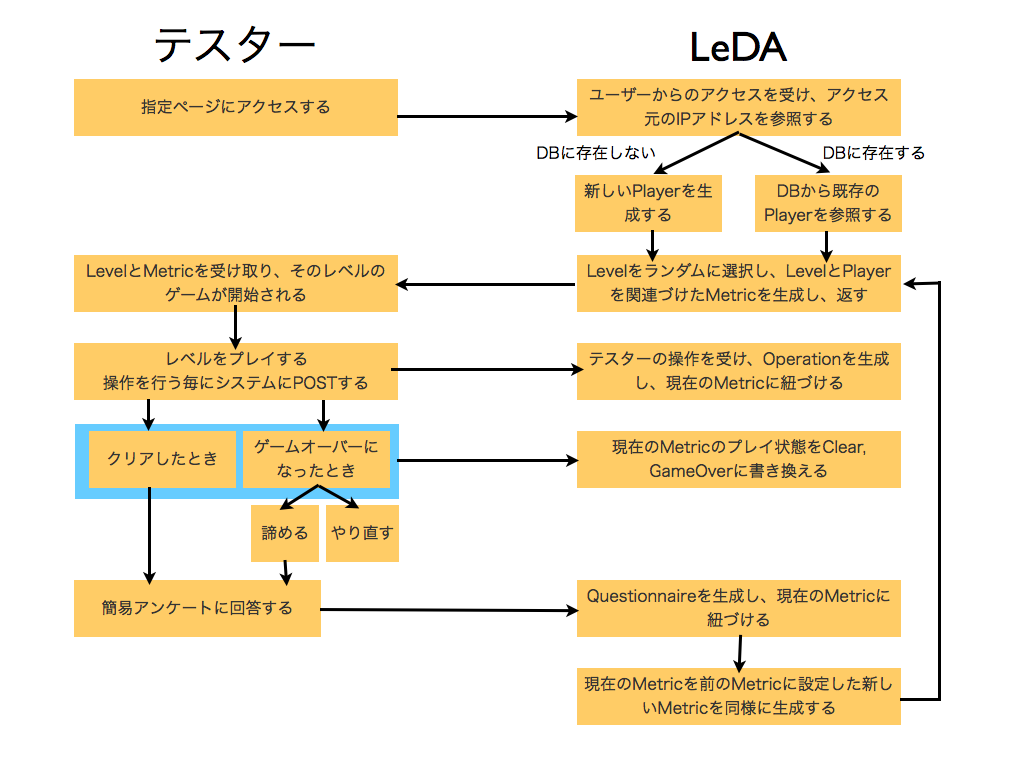
\includegraphics[bb=0 0 1024 768, width=15cm]{images/flow.png}
  \end{center}
  \caption{システムのフローチャート}
  \label{fig:one}
\end{figure}

\subsection{1. アクセス後の処理}
プレイヤーがWebブラウザにアクセスすると、プレイヤーのリクエストをシステムが受け、アクセス元のIPアドレスを参照する。

IPアドレスをDBから検索し、もし存在していなければ、そのアクセスが新規プレイヤーだと仮定し、新たなPlayerを生成し、DBに格納する。
もし、存在していれば、そのPlayerをDBから取得する。

その後、システムに登録されているLavelの中からランダムに1つを選択、LevelとPlayerを関連づけた新しいMetricを生成する。

このMetric1つ1つが1ゲーム分のログを表すデータである。

システムは生成されたMetricの主キーとLevelのデータをクライアントに返却する

\subsection{2. ゲームの開始}
サーバーからLevelのデータを受け取ると、ブラウザ上ではそのデータを元にLevelが再現され、即座にゲームが起動する。

プレイヤーはサーバーとの通信を意識することなくゲームをプレイすることができる。


\subsection{3. プレイヤー操作の記録}
プレイヤーのゲーム中での入力操作と現在のMetricの主キーが、操作を行う度にサーバーへ送信される。

サーバーはその情報を受け、受け取った入力操作を元にOperationを生成し、Metricに追加する。

この操作は、ゲーム終了まで何度も行われる。

\subsection{4. ゲーム状態の変化}
ゲーム中でプレイヤーがクリアやゲームオーバー状態に達したとき、その変化を現在のMetricの主キーと共にサーバーに送信する。

システムはその情報を受け、対応するMetricの状態を変更する。これによって、そのプレイの最終状態がどのような状態で終わったかをシステム管理者が容易に把握することができる。


\subsection{5. ゲームの終了}
プレイヤーがクリアする、または未クリアだがギブアップを選択したとき、プレイ後に何らかのアンケートが表示され、プレイヤーの声を収集することもできる。アンケートの結果はサーバーに送信され、
Questionnaireが生成され、現在のMetricと関連づけられる。


未クリアかつ、リプレイを選択した場合、アンケートは表示されずに、1のステップへ戻り、ランダムに選択されたLevelではなく、現在と同様のLevelが再び配信される。
また、現在のMetricが次に生成されるMetricに関連づけられる。

\subsection{6. 次のゲームの開始}
5までのステップで、一連のプレイログの記録が終了し、ここまでのデータを一つのMetricとして扱う。

プレイヤーが他のレベルに挑戦したい場合、再び1の手順とほぼ同様の処理が行われ、新たなLevelの配信と、Metricの生成が行われる。

このとき、必ず現在遊んだLevelと異なったLevelが配信されてくる。また、次に新しく生成されるMetricの前のMetricとして、現在のMetricが関連づけられる。


\section{実装}
実装は主にサーバーサイドとクライアントサイドに分かれて行われている。

\subsection{サーバーサイド}
サーバーサイドの実装は、Python製のWeb Application FrameworkであるDjangoにより実装されている。このFrameworkはOSSであり、簡単に利用できる。

このFrameworkにより実装されたシステムを、Apache上でPythonを動作させるモジュール、mod\_wsgiを用いてサーバー上で動作させている。

また、アプリケーション上で生成されたモデルを格納するリレーショナル・データベースは、取り扱いの容易さの観点からsqlite3を採用している。

\subsection{クライアントサイド}
クライアントサイドでは、ゲームロジックがJavaScriptで記述され、HTML5のCanvasタグにより描画されている。

またJavaScriptのソースコードは、メタ言語であるCoffeeScriptで記述されている。

その他、サーバーとクライアントの通信に、JavaScript製ライブラリであるjQueryを利用している。
サーバーとのデータ通信は、サーバーのアプリケーション上にあるモデルをJSONというデータ記述言語としてダンプし、その文字列をやりとりすることにより行っている。

\renewcommand{\bibname}{参考文献}
\begin{thebibliography}{10}
\bibitem{metrics} University of Copengagen, Anders Drachen, Alessandro Canossa, Towards Gameplay Analysis via Gameplay Metrics
\bibitem{usability} Desurvire, Heather Wiberg, Charlotte, Game Usability Heuristics ( PLAY ) for Evaluating and Designing Better Games : The Next Iteration \bibitem{mario} Infinite Mario Bros http://www.mojang.com/notch/mario/ \bibitem{model} University of Copenhagen, Chris Pedersen, Julian Togelius, Georgios Yannakakis, Modeling player experiece in Super Mario Bros.
\bibitem{optimization} University of Copenhagen, Chris Pedersen, Julian Togelius, Georgios Yannakakis, Optimization of Platform Game Level for Player Experience
\bibitem{level} Shaker, Noor Togelius, Julian Yannakakis, Georgios N.  Weber, Ben Shimizu, Tomoyuki Hashiyama, Tomonori Sorenson, Nathan Pasquier, Philippe Mawhorter, Peter Takahashi, Glen Smith, Gillian Baumgarten, Robin The 2010 Mario AI Championship: Level Generation Track
\bibitem{champion} Mario AI Championship http://www.marioai.org/
\bibitem{ga} はこだて未来大学 五木宏 松原仁 遺伝アルゴリズムの視覚化を用いたゲームのレベルデザイン効率化技法の開発
\bibitem{auto} Togelius, Julian Schmidhuber, Jurgen An experiment in automatic game design
\bibitem{gamedesign} Georgia Institute of Technology Nelson, Mark J Mateas, Michael Towards Automated Game Design
\end{thebibliography}

\end{document}
